\documentclass[a4paper,12pt]{article}
\usepackage[utf8]{inputenc}
\usepackage[T1]{fontenc}
\usepackage[hungarian]{babel}
\usepackage{graphicx}
\usepackage{geometry}
\geometry{a4paper,
		     tmargin = 35mm, 
		     lmargin = 25mm,
		     rmargin = 30mm,
		     bmargin = 30mm}
\usepackage{mathtools}
\usepackage{amsmath}
\usepackage{color}
\usepackage{setspace}
\usepackage{amsmath,amssymb}
\usepackage{float}


\usepackage{indentfirst}
\usepackage{subfig}

\renewcommand\thesection{\Roman{section}}

\begin{document}

\linespread{1.2}

\begin{titlepage}

	\centering
	
\includegraphics[width=0.66\textwidth]{../elte.jpg}\par\vspace{1cm}
	{\scshape\LARGE ELTE TTK \par}
	\vspace{3cm}
	{\scshape\Large Pásztázó elektronmikroszkópia\par}
	\vspace{1cm}
	{\large\itshape Olar Alex\par}
	\vspace{3cm}
	{\large 2018 \par}

\end{titlepage}

\begin{abstract}
	\par A mérés célja a SEM mikroszkóppal való ismerkedés és a tapasztalat szerzés volt. Idén láthattuk, hogy
	a modern technika eliminálta a laborok eddigi legfontosabb részét, avagy az 50 éves műszer kalibrálását és
	kezelését. Láthattuk, hogy egy modern géppel, a modern szoftverek szinte mindent megcsinálnak helyettünk.
\end{abstract}

\vfill

\tableofcontents

\newpage

\section{Elméleti összefoglaló}

\par A pásztázó elektronmikroszkópia elmélete már korábbi tanulmányaink során előfordult és a leírásban
is szerepel. A képkészítéshez a műszer a szekunder elektronokat és a visszaszórodott elektronokat használta
és a képeket a megfelelő elektronika készítette el a műszerben lévő detektor segítségével.

\section{A mérés lépései}

\par A mérés során a modern műszer lehetőve tette, hogy mindhárman válasszunk egy mintát és azt megvizsgáljuk.
Megvizsgáltuk Dávid ezüst láncát és két micro chipet amik demonstrációs célra voltak fenntartva. Adott mintáról
készítettünk röntgen spektroszkópiai felvételeket is, melynek segítségével meg tudtuk határozni a kellő program
segítségével az anyagösszetételt és az összetétel arányt is a felszín közelében. Ezeket a képeket közlöm majd a
megfelelő táblázatokkal.

\par Előszöris persze egy három anyagból álló (szilícium-titán-réz/nikkel ötvözet) mintát vizsgáltunk a fentebbi
módszerekkel, hogy megismerjük a műszert és annak használatát.

\vfill

\newpage

\section{Mérési eredmények}

\subsection{Első minta}

\begin{figure}[H]
	\centering
	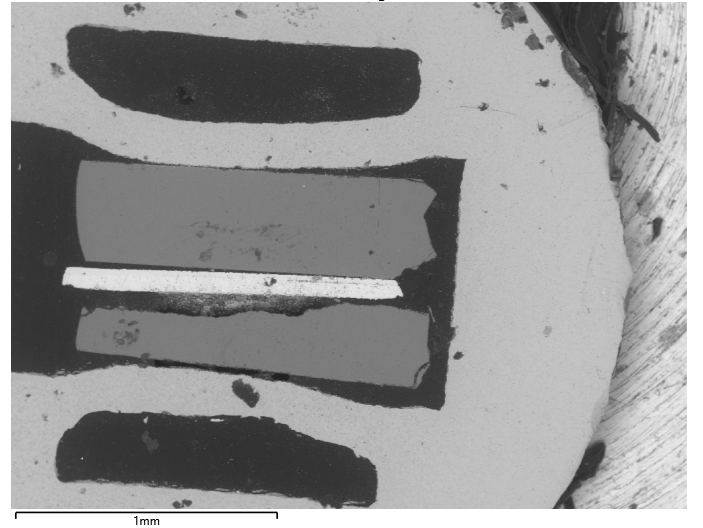
\includegraphics[width=0.35\textwidth, height=0.25\textwidth]{Jcsop/elso.png}
	\caption{Tanuló minta}
\end{figure}

\par A program által meghatározott anyagösszetétel is jól látható az alábbi ábrán. De a teljesség kedvéért
le is írom: Ni, Cu, Ti, Si, C.

\begin{figure}[H]
	\centering
	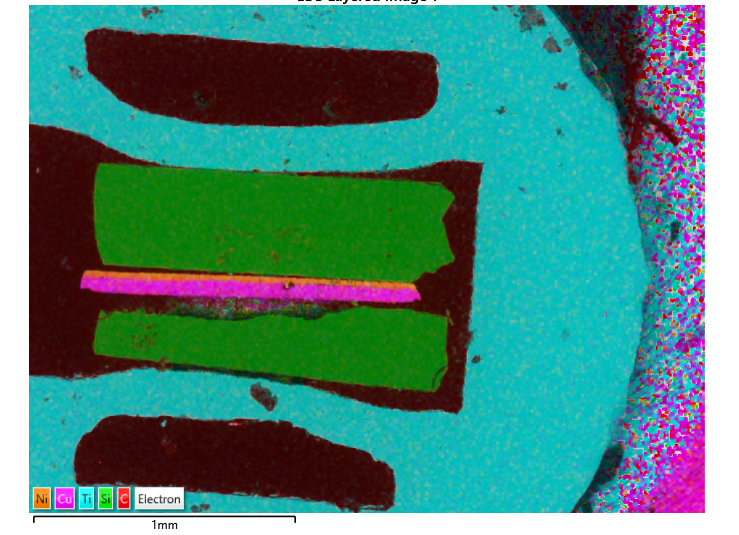
\includegraphics[width=0.65\textwidth, height=0.45\textwidth]{Jcsop/elsoanyag.png}
	\caption{Tanuló minta anyagösszetétele}
\end{figure}

\par Ugyan ezek az anyagok szépen szeparálódnak az egyenkénti röntgen felvételeken. A fentebbi kép ezek
szintetikus összerakásával készült:

\begin{figure}[H]
	\centering
	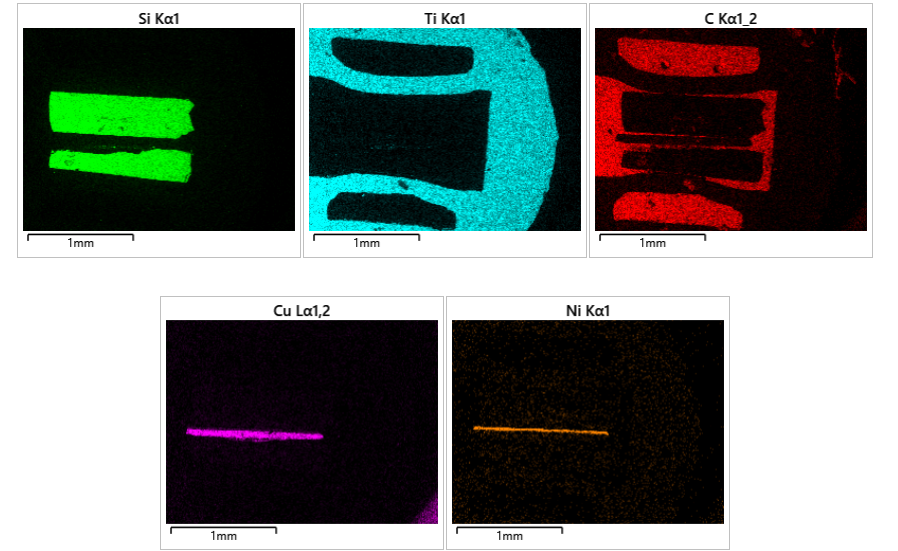
\includegraphics[width=0.65\textwidth, height=0.45\textwidth]{Jcsop/elsortg.png}
	\caption{Tanuló mintáról készült röntgen analízis}
\end{figure}

\subsubsection{Összetétel meghatározása}

\par Az alábbi mintáról a Cu L$\alpha$1,2 képet vizsgáltuk. A feladat
az volt, hogy a kapott képen márjük meg a különböző anyagok arányát (Cu-Ni-Si)
majd a készített hisztogrammon ezt ismételjük meg.

\begin{figure}[H]
	\centering
	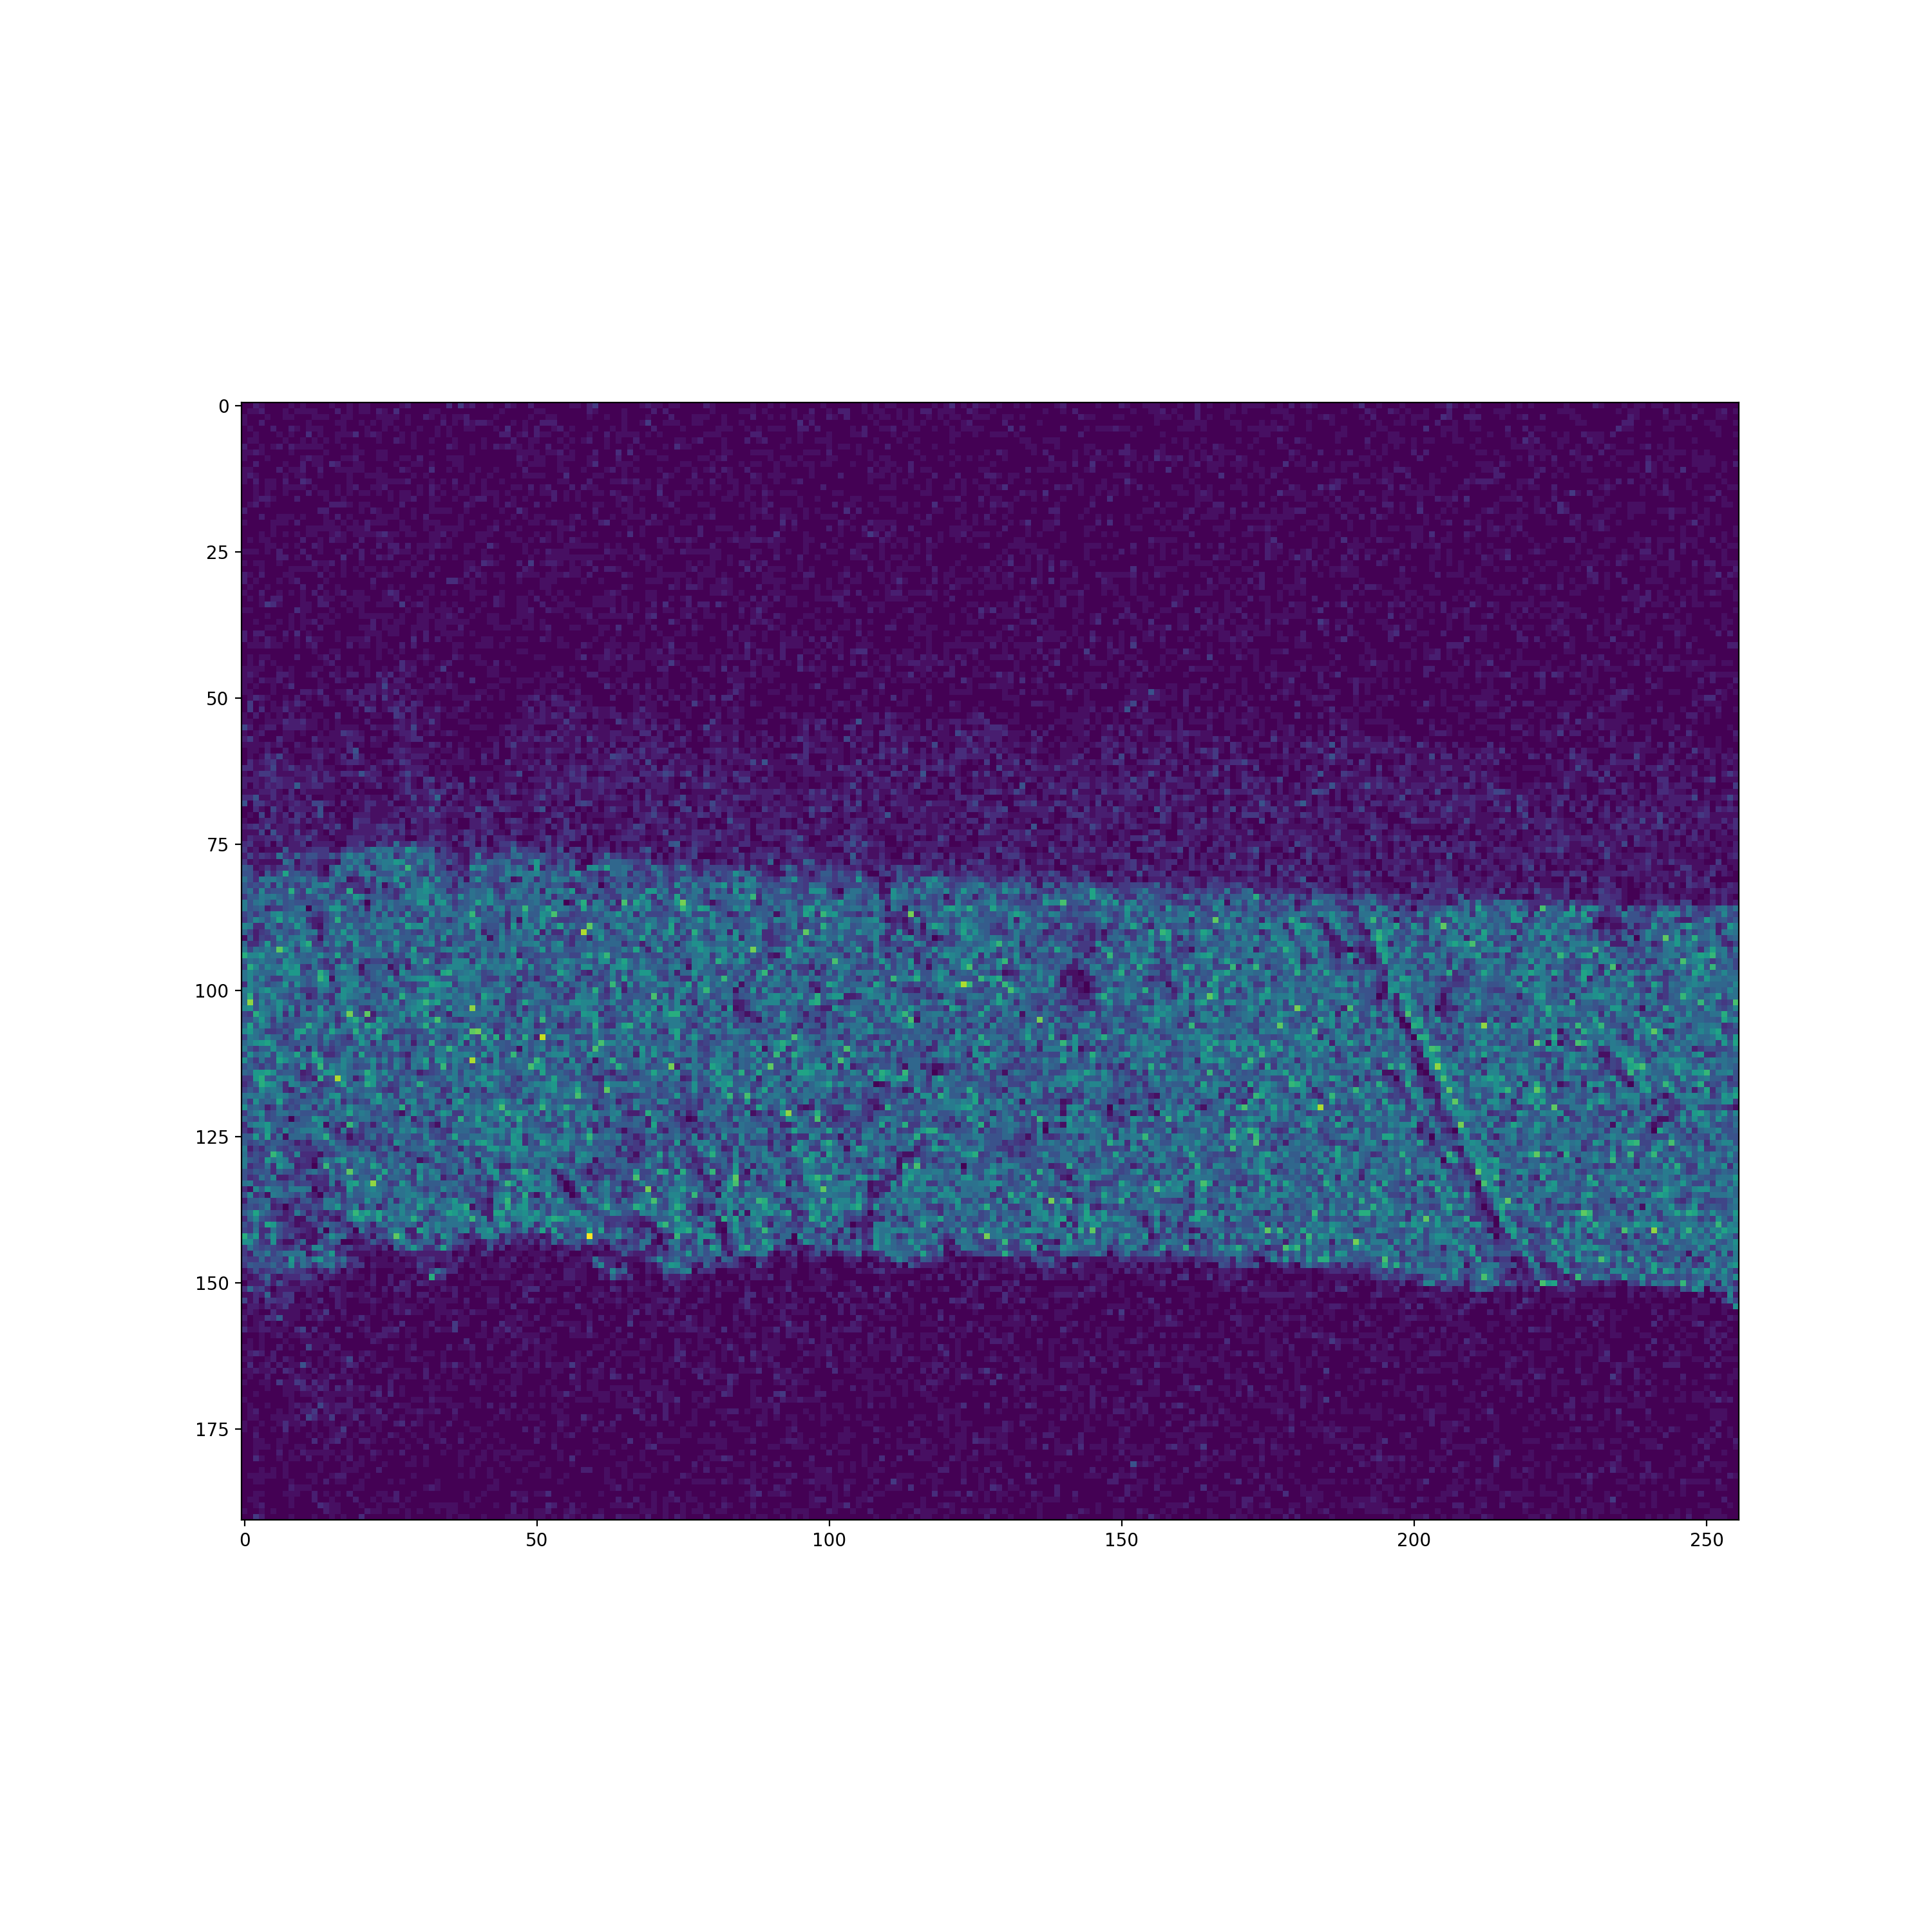
\includegraphics[width=0.52\textwidth]{histoimg.png}
	\caption{A vizsgált kép, a csv fájlból generálva.}
\end{figure}

\par A python matplotlib csomagjával az előbbi képből egy oszlop diagrammot
készítettem. Ennek a beosztását [0,20] közötti intervallumban vettem, hiszen a
kapott kép nem tartalmazott ennél nagyobb értékeket adott pixelben.

\begin{figure}[H]
	\centering
	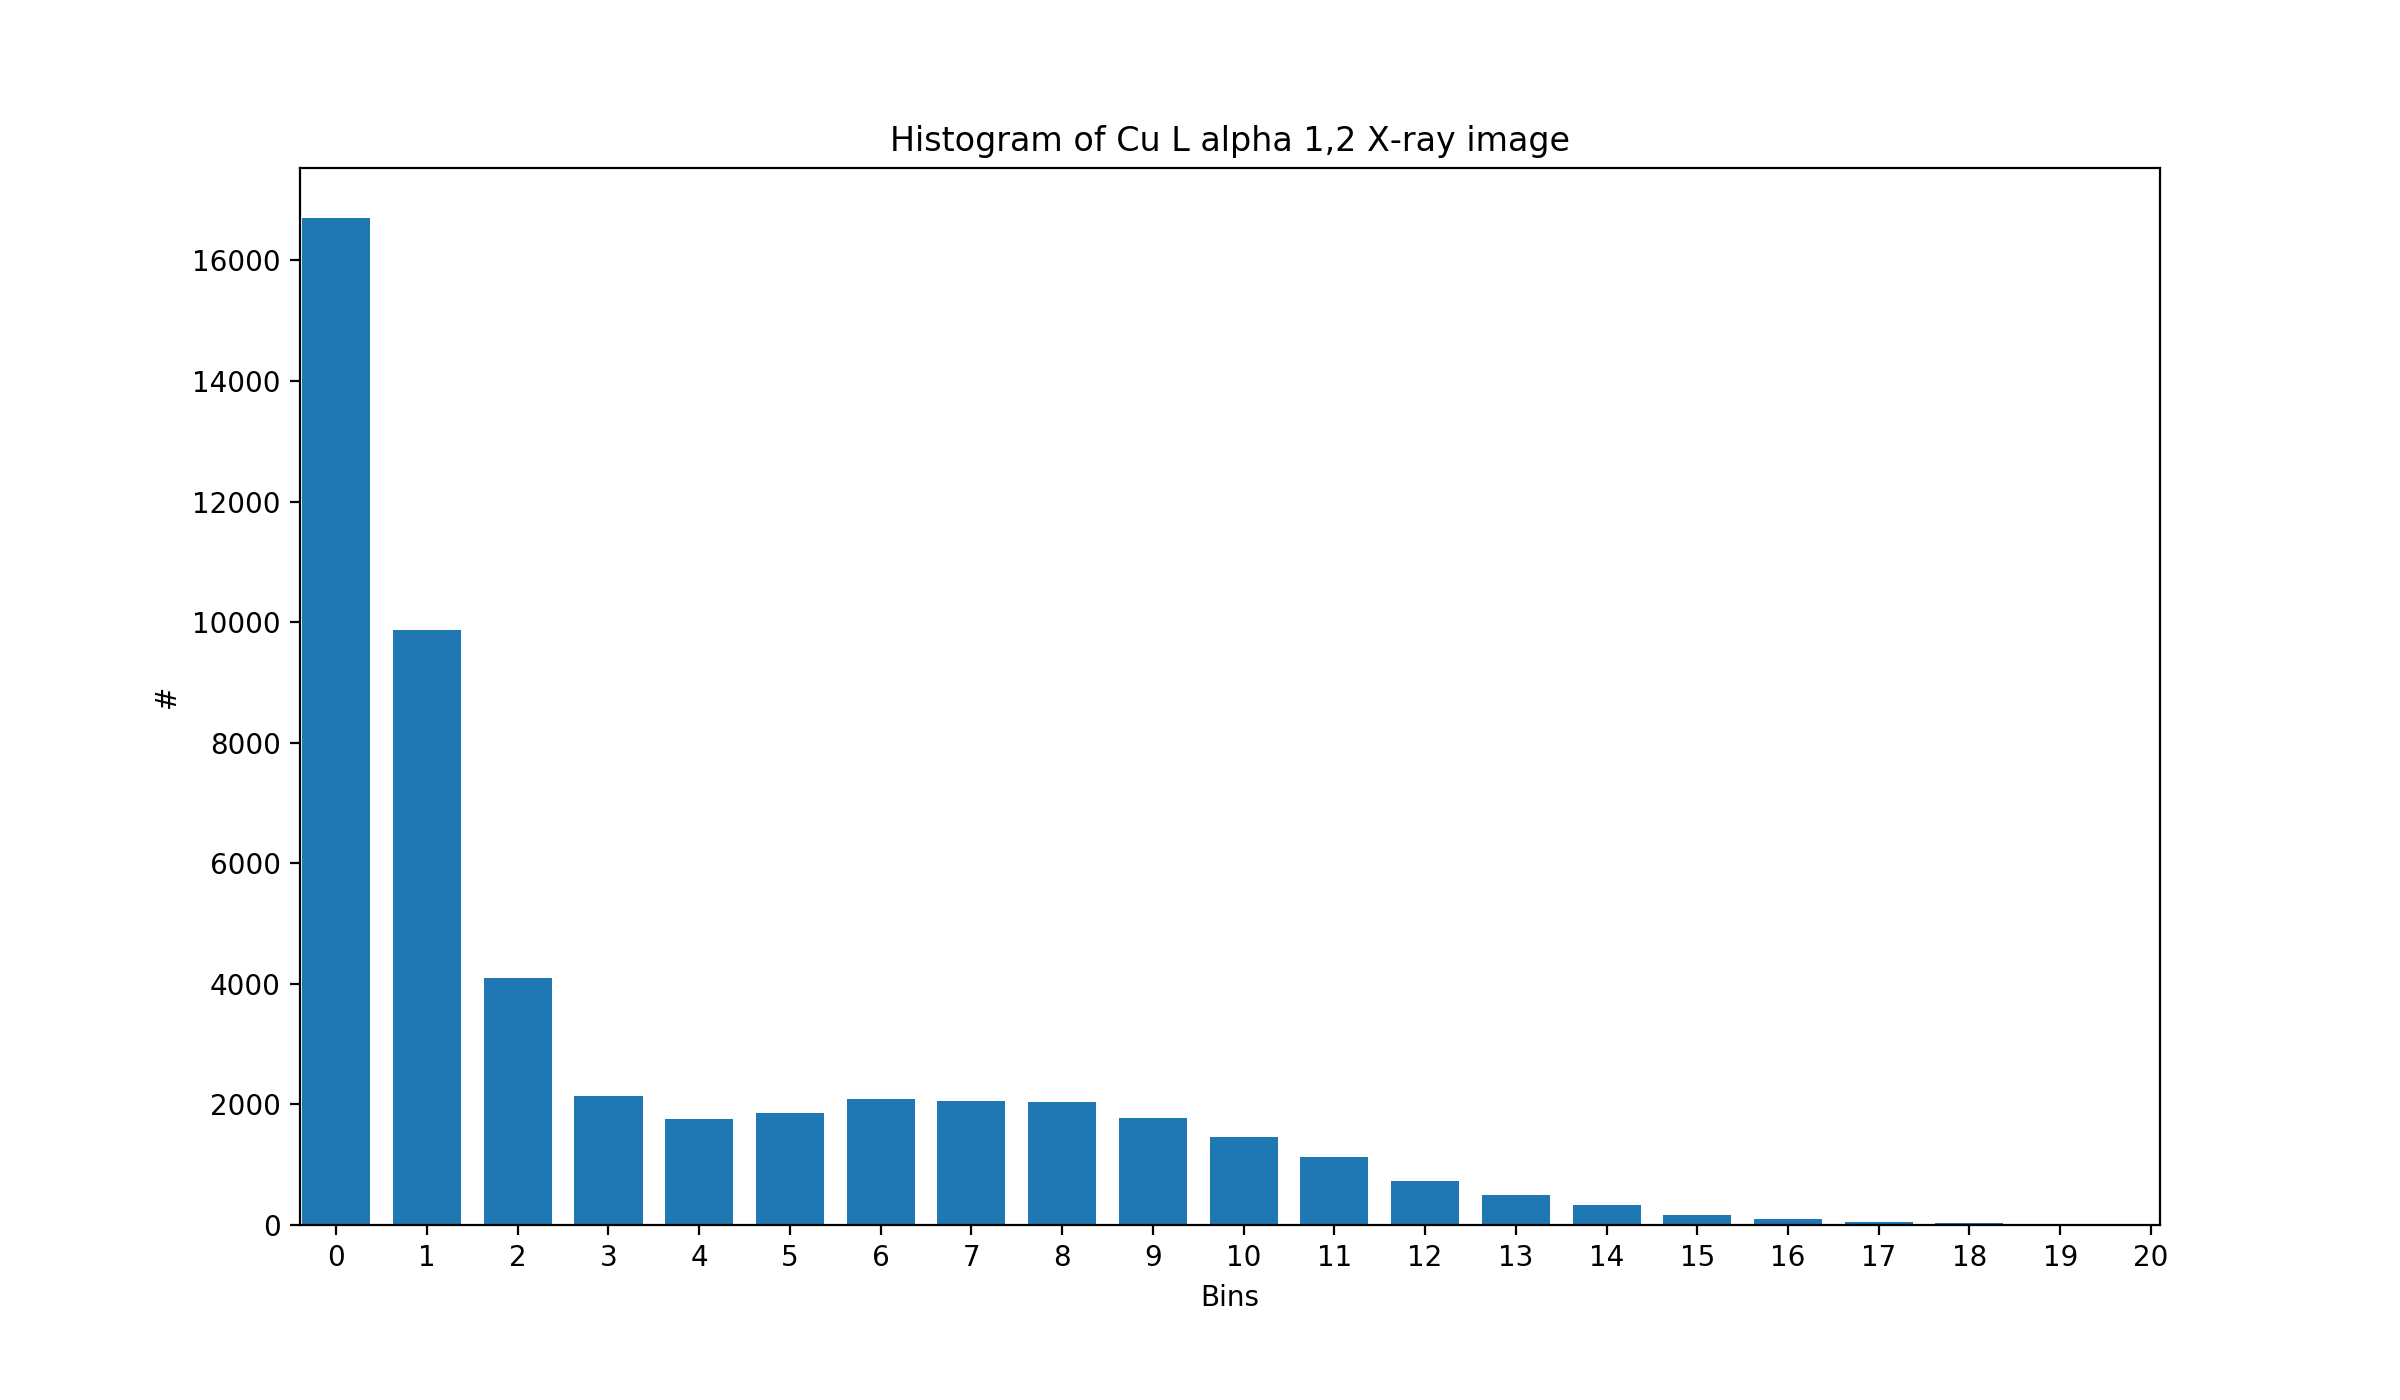
\includegraphics[width=0.82\textwidth]{histo.png}
	\caption{A kép hisztogrammon.}
\end{figure}

\par Jól látható, hogy a 192x256-os kép nagy része 0-ás értékű, ezeket veszem a legsötétebb
pontoknak. Nem jól elkülöníthatő a szemmel jól látható nikkel réteg a kép
közepe táján, ezt a kisebb csúcs előtti résznek veszem. Az eredmények a következők:

\begin{table}[H]
	\centering
	\begin{tabular}{|c|c|c|c|c|}  \hline
		-      & Measured & err    & Integrated & err    \\ \hline
		dark   & 165      & 24.75  & 16697      & 1669.7 \\ \hline
		mid    & 44       & 6.6    & 5756       & 575.6  \\ \hline
		bright & 126.5    & 18.975 & 12467      & 1246.7 \\ \hline
	\end{tabular}
	\caption{A felszíni anyagösszetétel eloszlása}
	\label{my-label}
\end{table}

\par Kézzel mért esetben a becsült hiba 15\%-os mivel képtelenség volt
pontosan meghatározni a színátmenetek határát. Ugyan ez a hiba 10\%-ra becsült
az integrált esetben, hiszen a 20 bin-es felosztás lehetővé teszi jól definiált határok
felállítását.

\par A sorok a legsötétebbtől a legvilágosabb kékig mennek. A legsötétebbhez
viszonyítva (*/dark - mért vagy integrált ):

\begin{table}[H]
	\centering
	\begin{tabular}{|c|c|c|c|}  \hline
		- & dark/dark & mid/dark & bright/dark \\ \hline
		Integrated  & - & 0.34472 $\pm$ 0.0345 & 0.74667 $\pm$ 0.0747 \\ \hline
		Measured & - & 0.2667 $\pm$ 0.04 & 0.7667 $\pm$ 0.1150 \\ \hline
	\end{tabular}
	\caption{A felszíni anyagösszetétel eloszlása}
	\label{my-label}
\end{table}

\par Jól látható, hogy a legvilágosabb rész jól elkülönítható, míg a 
közepesen világos rész hibahatáron nem egyezik meg. Ez nem meglepő, hiszen
alig alig elkülöníthatő a széle a sötét és a világos rész közötti közepes
átmenethez.

\subsection{Ezüst lánc}

\par Közlöm a készített képeket:

\begin{figure}[H]
	\centering
	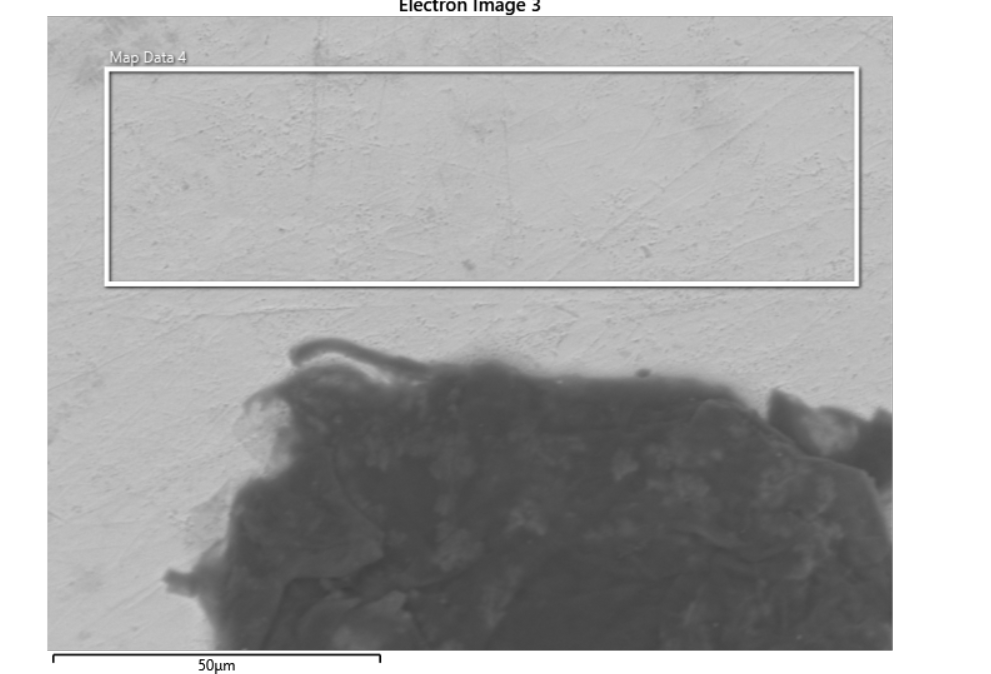
\includegraphics[width=0.62\textwidth]{./Jcsop/lanc.png}
	\caption{SEM kép, a később röntgennel vizsgált terület jelölve.}
\end{figure}

\begin{figure}[H]
	\centering
	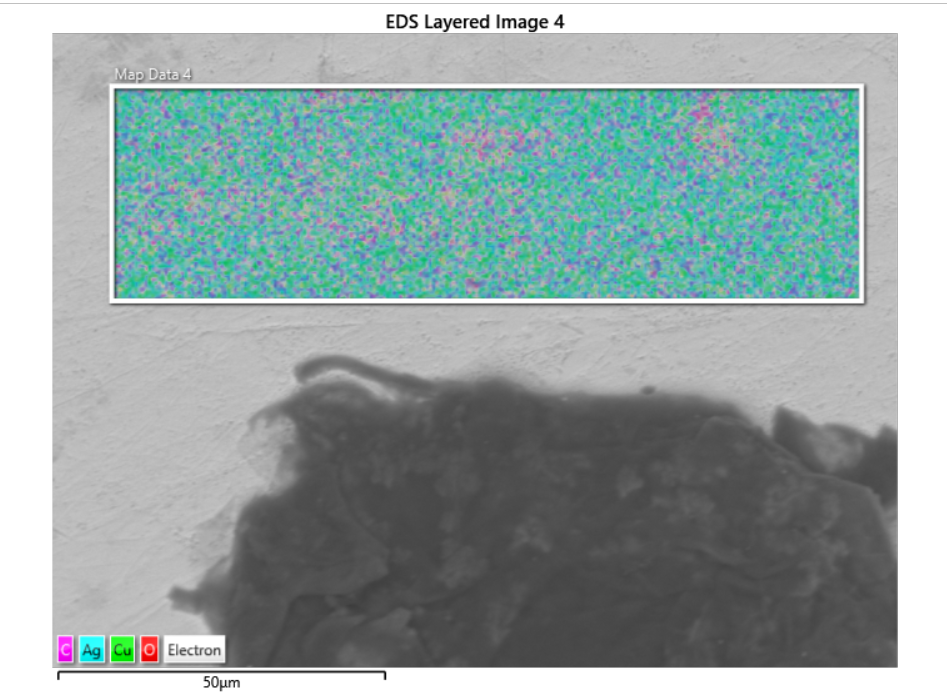
\includegraphics[width=0.62\textwidth]{./Jcsop/lancrtg.png}
	\caption{SEM kép, röntgen összetétel analízis.}
\end{figure}

\par Az anyagösszetételt százalékosan, relatív hibákkal közlöm:

\begin{table}[H]
	\centering
	\begin{tabular}{|c|c|c|}  \hline
		Element & Weight [\%] & $\sigma$ \\ \hline
		Ag      & 81.6        & 0.3      \\ \hline
		O       & 5.5         & 0.1      \\ \hline
		C       & 4.9         & 0.2      \\ \hline
		Cu      & 4.1         & 0.1      \\ \hline
		Cd      & 2.1         & 0.2      \\ \hline
		Na      & 0.7         & 0.1      \\ \hline
		Zn      & 0.7         & 0.1      \\ \hline
		Cl      & 0.3         & 0.0      \\ \hline
		Al      & 0.2         & 0.0      \\ \hline
		Si      & 0.1         & 0.0      \\ \hline
	\end{tabular}
	\caption{A felszíni anyagösszetétel eloszlása}
	\label{my-label}
\end{table}

\subsection{Micro chip}

\subsubsection{Demonstrációs chip 1.}

\par Az alábbi esetben nem volt külön feladat, csak a képeket közlöm.

\begin{figure}[H]
	\centering
	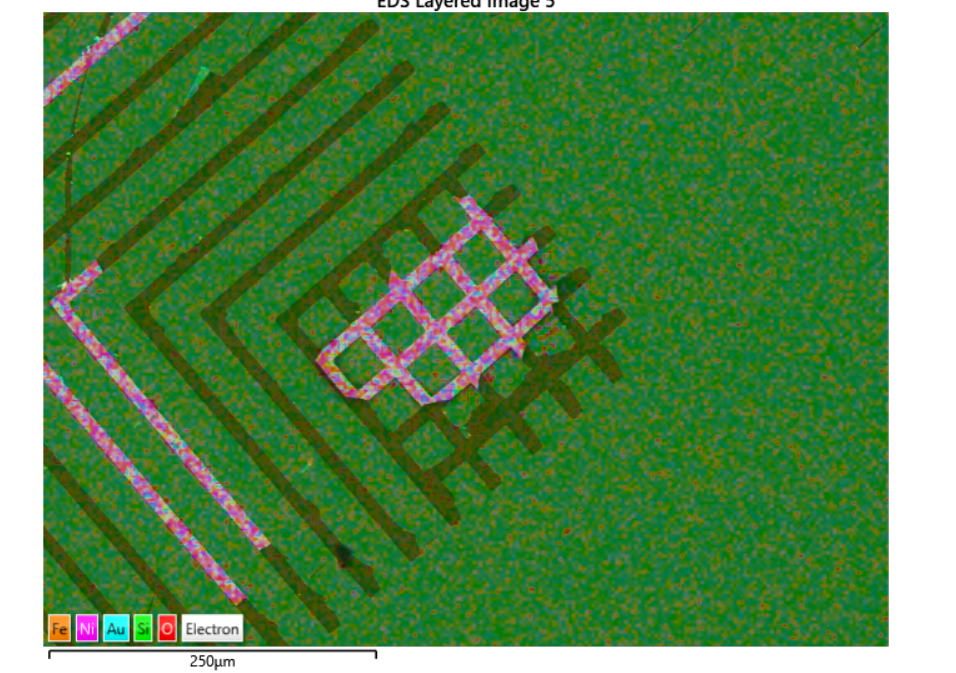
\includegraphics[width=0.7\textwidth]{./Jcsop/chip1.png}
	\caption{SEM kép, röntgen analízis után szintetikusan színezve}
\end{figure}

\begin{figure}[H]
	\centering
	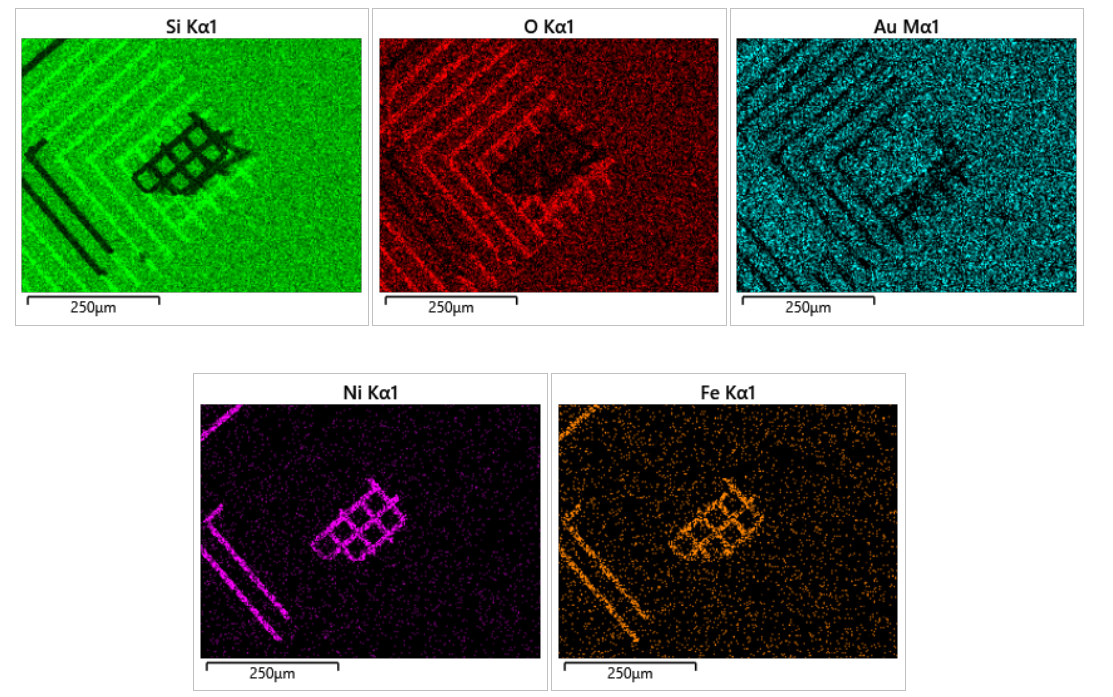
\includegraphics[width=0.6\textwidth]{./Jcsop/chip1rtg.png}
	\caption{SEM kép, röntgen összetétel analízis.}
\end{figure}

\par Az anyagösszetételt százalékosan, relatív hibákkal közlöm:

\begin{table}[H]
	\centering
	\begin{tabular}{|c|c|c|} \hline
		Element & Weight \% & $\sigma$ \\  \hline
		Si      & 49.1      & 0.2      \\ \hline
		O       & 24.7      & 0.2      \\ \hline
		Au      & 13.7      & 0.2      \\ \hline
		C       & 8.2       & 0.3      \\ \hline
		Ni      & 3.5       & 0.1      \\ \hline
		Fe      & 0.9       & 0.1      \\ \hline
	\end{tabular}
	\caption{A felszíni anyagösszetétel eloszlása}
\end{table}

\subsubsection{Demonstrációs chip 2.}

\par Az utolsó chipnél, le kellett mérni a beosztások méretét és
megkeresni az összefüggést a jelzett számokkal.

\begin{figure}[H]
	\centering
	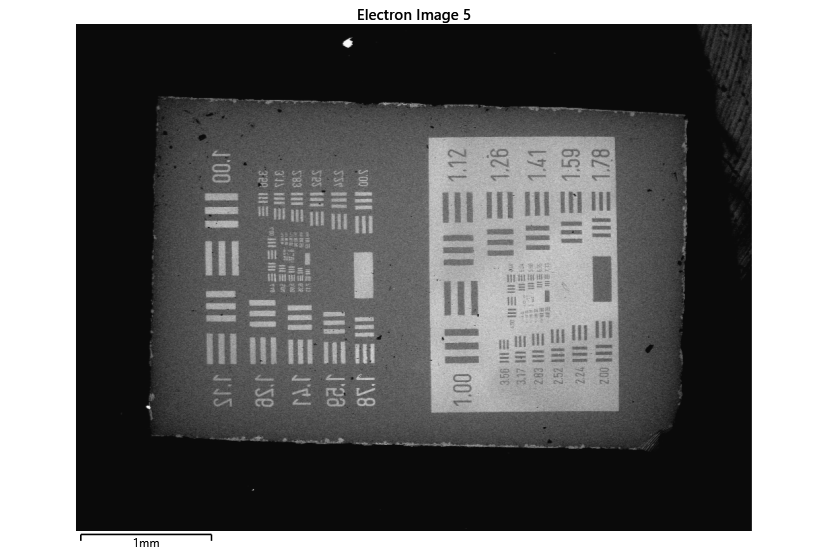
\includegraphics[width=0.75\textwidth]{./Jcsop/chip2.png}
	\caption{SEM kép}
\end{figure}

\begin{figure}[H]
	\centering
	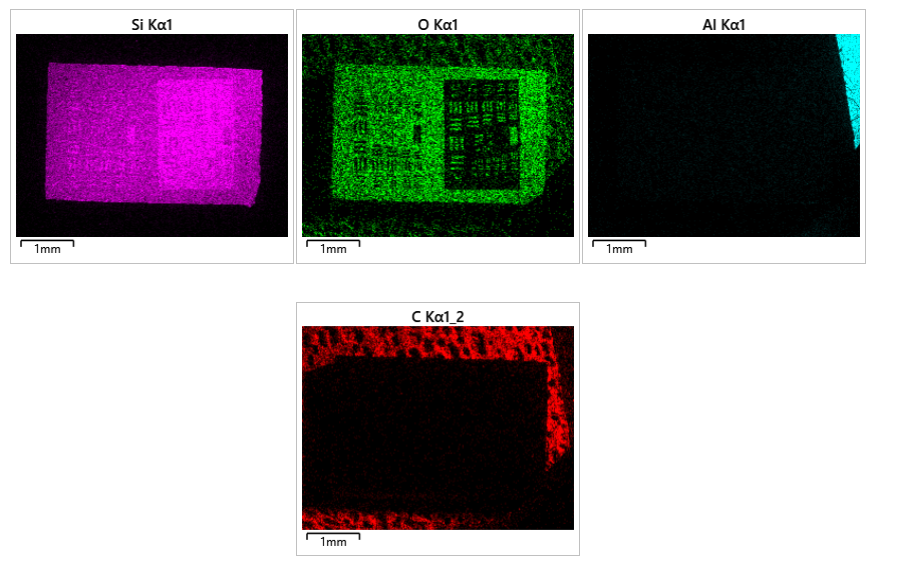
\includegraphics[width=0.66\textwidth]{./Jcsop/chip2rtg.png}
	\caption{SEM kép, röntgen összetétel analízis.}
\end{figure}

\section{Összefoglalás}



\end{document}